\documentclass[12pt,twoside]{report}
\usepackage{graphicx}
\usepackage{alphalph}
\usepackage{subcaption}
\usepackage[a5paper,margin=1cm]{geometry}
\renewcommand*{\thesubfigure}{(\arabic{subfigure})}
\begin{document}
\begin{figure}
\centering
\begin{subfigure}[b]{0.20\textwidth}
\centering

\includegraphics[width=\textwidth]{../../trajectories/264.png}
\caption{Id:264}
\end{subfigure}
\begin{subfigure}[b]{0.20\textwidth}
\centering
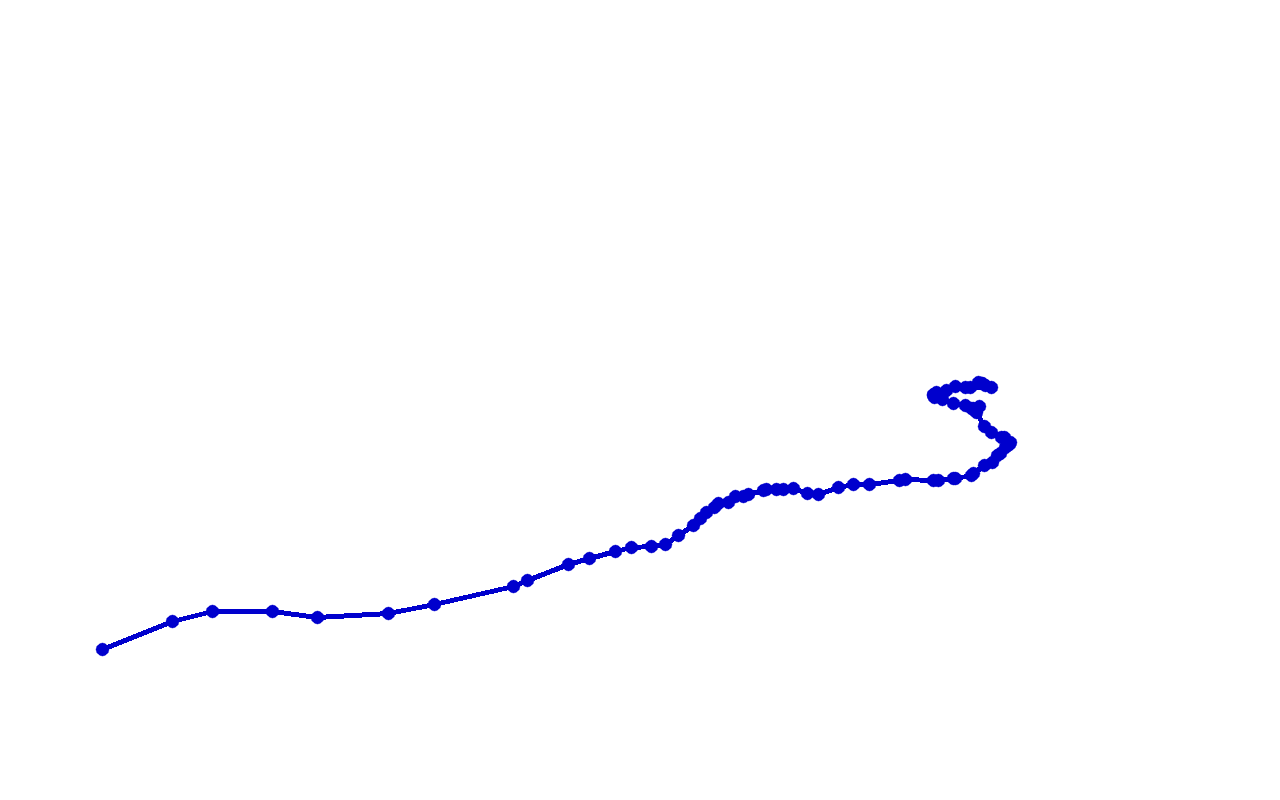
\includegraphics[width=\textwidth]{../../trajectories/480.png}
\caption{Id:480}
\end{subfigure}
\begin{subfigure}[b]{0.20\textwidth}
\centering

\includegraphics[width=\textwidth]{../../trajectories/522.png}
\caption{Id:522}
\end{subfigure}
\begin{subfigure}[b]{0.20\textwidth}
\centering
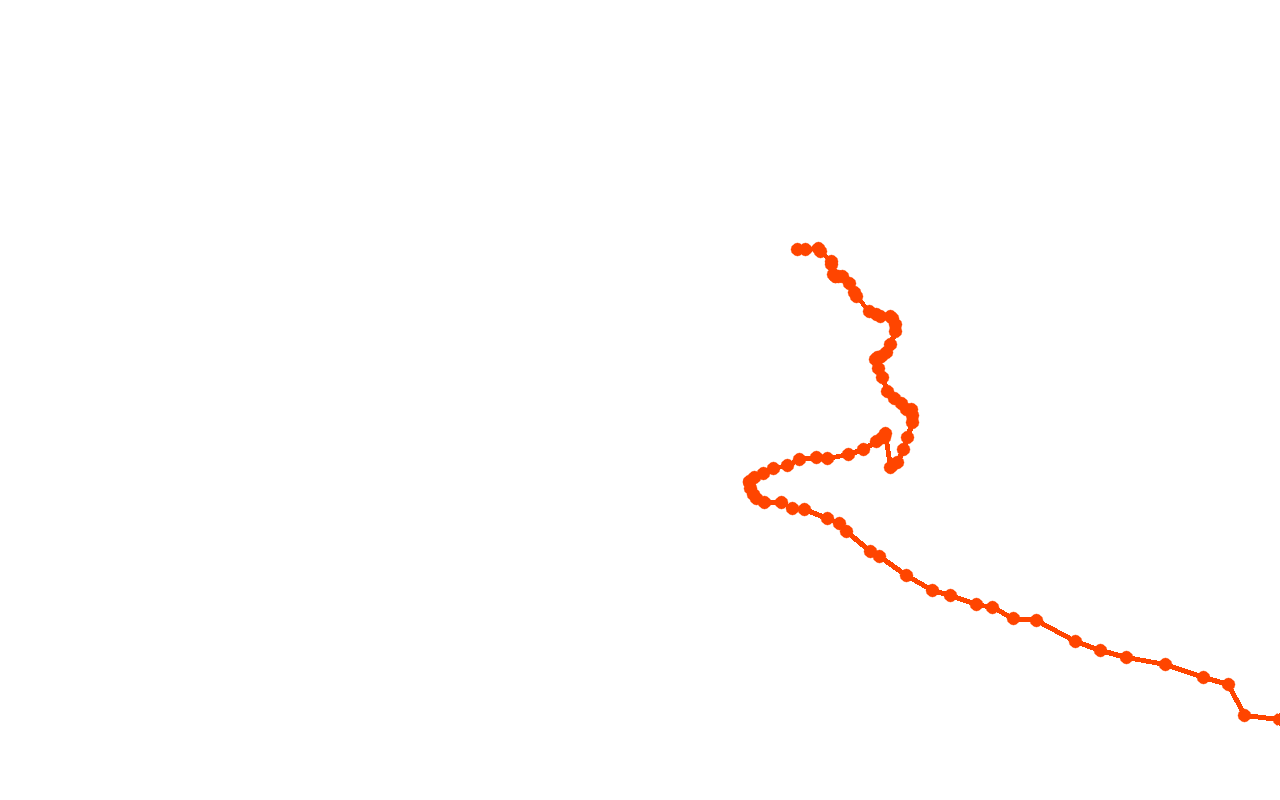
\includegraphics[width=\textwidth]{../../trajectories/744.png}
\caption{Id:744}
\end{subfigure}
\begin{subfigure}[b]{0.20\textwidth}
\centering

\includegraphics[width=\textwidth]{../../trajectories/761.png}
\caption{Id:761}
\end{subfigure}
\begin{subfigure}[b]{0.20\textwidth}
\centering

\includegraphics[width=\textwidth]{../../trajectories/862.png}
\caption{Id:862}
\end{subfigure}
\end{figure}
\end{document}